\documentclass[aspectratio=169,9pt,t]{beamer}

\usepackage{graphicx}
\usepackage{tikz}
\usetikzlibrary{arrows.meta, positioning, decorations.pathreplacing}
\usepackage{listings}
\usepackage{xcolor}
\usepackage{hyperref}
\usepackage{tabularx}

% Remove navigation symbols
\usepackage{etoolbox}
\apptocmd{\itemize}{\setlength{\itemsep}{1.5pt}\setlength{\topsep}{1pt}}{}{}
\apptocmd{\enumerate}{\setlength{\itemsep}{2pt}\setlength{\topsep}{1pt}}{}{}
\setbeamertemplate{navigation symbols}{}

% ---------- Slide counter (frame number / total) ----------
\setbeamertemplate{footline}{
    \vbox to 0.75cm{\vfil\hbox to \paperwidth{\hfill\insertframenumber~/~\inserttotalframenumber\hspace{4pt}}\vspace{3pt}}
}

% ---------- Custom title page (shifted down, black text, bigger title) ----------
\setbeamertemplate{title page}{
    \vspace{2.5cm}
    \begin{center}
        {\color{black}\Huge\bfseries\inserttitle}\\[0.5cm]
        {\color{black}\normalsize\insertauthor}\\[0.2cm]
        {\color{black}\small\insertinstitute}\\[0.2cm]
        {\color{black}\small\insertdate}
    \end{center}
}

% ---------- Slide title shifted down and to the right ----------
\makeatletter
\setbeamertemplate{frametitle}{
    \vspace{0.4cm}
    \hspace{0.1cm}\insertframetitle
    \ifx\insertframesubtitle\@empty\else
        \par\vspace{0.05cm}\hspace{0.1cm}{\normalfont\small\itshape\color{qsgray}\insertframesubtitle}
    \fi
}
\makeatother

% ---------- Code listing styles ----------
\definecolor{codebg}{RGB}{245,245,245}
\definecolor{codegreen}{RGB}{0,128,0}
\definecolor{codepurple}{RGB}{128,0,128}
\definecolor{codeblue}{RGB}{0,0,180}
\definecolor{codeorange}{RGB}{204,102,0}

\lstset{
    basicstyle=\ttfamily\tiny,
    backgroundcolor=\color{codebg},
    frame=single,
    framerule=0.5pt,
    rulecolor=\color{gray},
    breaklines=true,
    breakatwhitespace=true,
    showstringspaces=false,
    tabsize=4,
    captionpos=b,
    xleftmargin=2pt,
    xrightmargin=2pt,
    aboveskip=4pt,
    belowskip=4pt,
}

\lstdefinestyle{bash}{
    language=bash,
    keywordstyle=\color{codeblue}\bfseries,
    stringstyle=\color{codegreen},
    commentstyle=\color{gray}\itshape,
    morekeywords={cd,git,clone,make,mkdir,curl,pixi,find,mv,ls},
}

\lstdefinestyle{python}{
    language=Python,
    keywordstyle=\color{codeblue}\bfseries,
    stringstyle=\color{codegreen},
    commentstyle=\color{gray}\itshape,
    emphstyle=\color{codepurple},
}

\lstdefinestyle{json}{
    language=,
    stringstyle=\color{codegreen},
    morestring=[b]",
    literate=
        *{0}{{{\color{codeorange}0}}}{1} {1}{{{\color{codeorange}1}}}{1}
         {2}{{{\color{codeorange}2}}}{1} {3}{{{\color{codeorange}3}}}{1}
         {4}{{{\color{codeorange}4}}}{1} {5}{{{\color{codeorange}5}}}{1}
         {6}{{{\color{codeorange}6}}}{1} {7}{{{\color{codeorange}7}}}{1}
         {8}{{{\color{codeorange}8}}}{1} {9}{{{\color{codeorange}9}}}{1},
}

\lstdefinestyle{http}{
    language=,
    basicstyle=\ttfamily\scriptsize,
    commentstyle=\color{gray}\itshape,
    morecomment=[l]{\#},
}

% ---------- Palette ----------
\definecolor{qsnavy}{RGB}{0,51,102}
\definecolor{qsblue}{RGB}{0,118,190}
\definecolor{qsteal}{RGB}{0,128,128}
\definecolor{qsgreen}{RGB}{46,125,50}
\definecolor{qsamber}{RGB}{200,120,0}
\definecolor{qsred}{RGB}{178,34,34}
\definecolor{qsgray}{RGB}{110,110,110}
\definecolor{qslight}{RGB}{235,241,247}
\definecolor{qslegacy}{RGB}{242,236,226}

\setbeamercolor{structure}{fg=qsnavy}
\setbeamercolor{frametitle}{fg=qsnavy}
\setbeamerfont{frametitle}{size=\Large,series=\bfseries}
\setbeamertemplate{blocks}[rounded][shadow=false]
\setbeamercolor{block title}{bg=qsnavy,fg=white}
\setbeamercolor{block body}{bg=qslight,fg=black}
\setbeamercolor{block title alerted}{bg=qsamber,fg=white}
\setbeamercolor{block body alerted}{bg=qslegacy,fg=black}
\setbeamercolor{block title example}{bg=qsgreen,fg=white}
\setbeamercolor{block body example}{bg=qslight,fg=black}
\setbeamertemplate{itemize items}[circle]
\setbeamertemplate{enumerate items}[default]
\setbeamersize{text margin left=0.9cm,text margin right=0.7cm}

% ---------- TikZ ----------
\usetikzlibrary{shapes.geometric, fit, calc, backgrounds, shadows}
\tikzset{
    box/.style={draw=qsnavy, thick, rounded corners=2pt, fill=white, align=center,
                font=\footnotesize, minimum height=0.8cm, inner sep=4pt},
    legacybox/.style={box, draw=qsamber, fill=qslegacy},
    store/.style={cylinder, shape border rotate=90, draw=qsnavy, thick, fill=white,
                  aspect=0.25, align=center, font=\footnotesize, minimum height=0.9cm, inner sep=3pt},
    legacystore/.style={store, draw=qsamber, fill=qslegacy},
    ext/.style={box, draw=qsgray, dashed, fill=white},
    arrow/.style={-{Stealth[length=2mm]}, thick, qsnavy},
    legacyarrow/.style={-{Stealth[length=2mm]}, thick, qsamber},
    both/.style={{Stealth[length=2mm]}-{Stealth[length=2mm]}, thick},
    lbl/.style={font=\tiny, fill=white, inner sep=1pt, text=qsgray},
    state/.style={draw=qsnavy, thick, rounded corners=3pt, fill=white, font=\footnotesize,
                  minimum height=0.7cm, minimum width=1.9cm, align=center},
    good/.style={state, draw=qsgreen, fill=qsgreen!10},
    bad/.style={state, draw=qsred, fill=qsred!8},
    stop/.style={state, draw=qsamber, fill=qsamber!10},
}

% ---------- Helpers ----------
\newcommand{\divider}[2]{%
    \dividerbackground
    \begin{frame}[plain]
        \vspace{2.9cm}
        \begin{center}
            {\color{qsnavy}\Huge\bfseries #1}\\[0.5cm]
            {\color{qsgray}\large #2}
        \end{center}
    \end{frame}
    \normalbackground
}
\newcommand{\src}[1]{{\color{qsgray}\tiny\texttt{#1}}}
\newcommand{\legacy}{QueueServer 0.x}
\newcommand{\vtwo}{V2}
\newcommand{\yes}{{\color{qsgreen}\(\checkmark\)}}
\newcommand{\no}{{\color{qsred}\(\times\)}}
\newcommand{\partly}{{\color{qsamber}\(\sim\)}}
\newcommand{\code}[1]{\texttt{#1}}
\usepackage{amssymb}
\usepackage{booktabs}
\usepackage{array}
\newcolumntype{L}[1]{>{\raggedright\arraybackslash}p{#1}}

% ---------- Background for title slide ----------
\newcommand{\titlebackground}{
    \usebackgroundtemplate{
        
\includegraphics[width=\paperwidth,height=\paperheight]{assets/NSLS2_Header.jpg}
    }
}

% ---------- Background for all other slides ----------
\newcommand{\normalbackground}{
    \usebackgroundtemplate{
        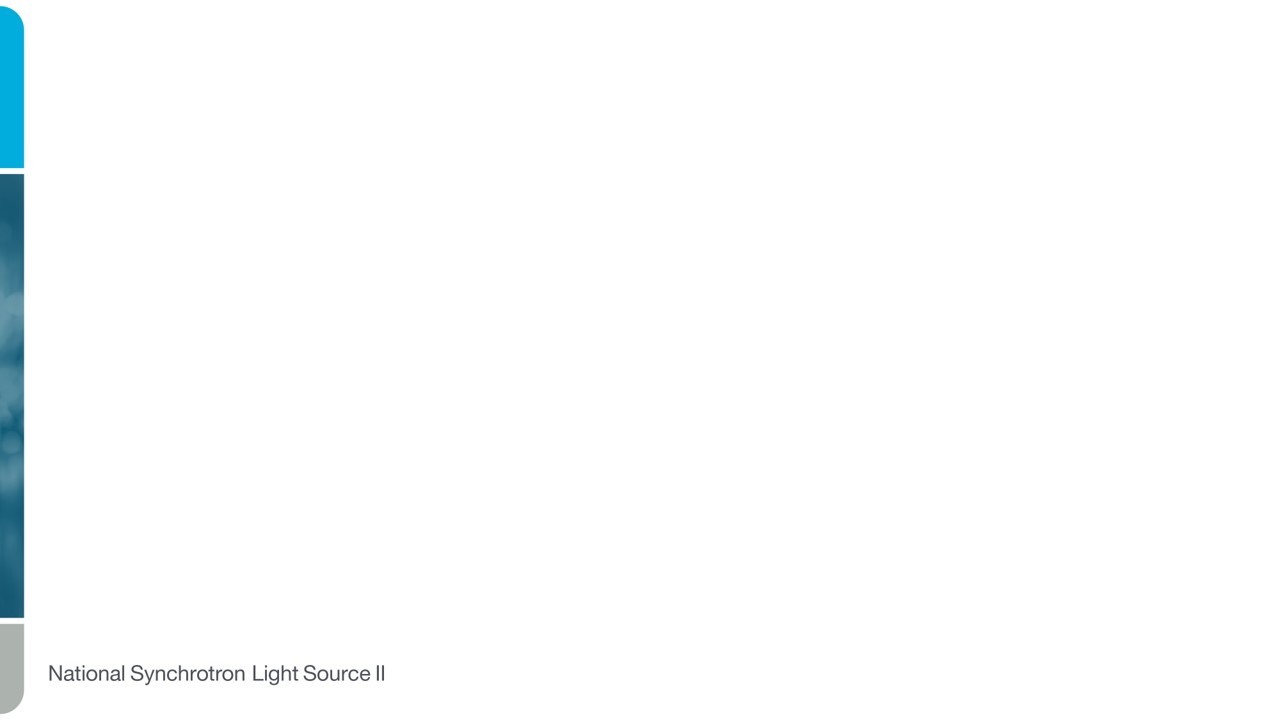
\includegraphics[width=\paperwidth,height=\paperheight]{assets/NSLS2_BG.jpg}
    }
}

% ---------- Background for section divider slides ----------
\newcommand{\dividerbackground}{
    \usebackgroundtemplate{
        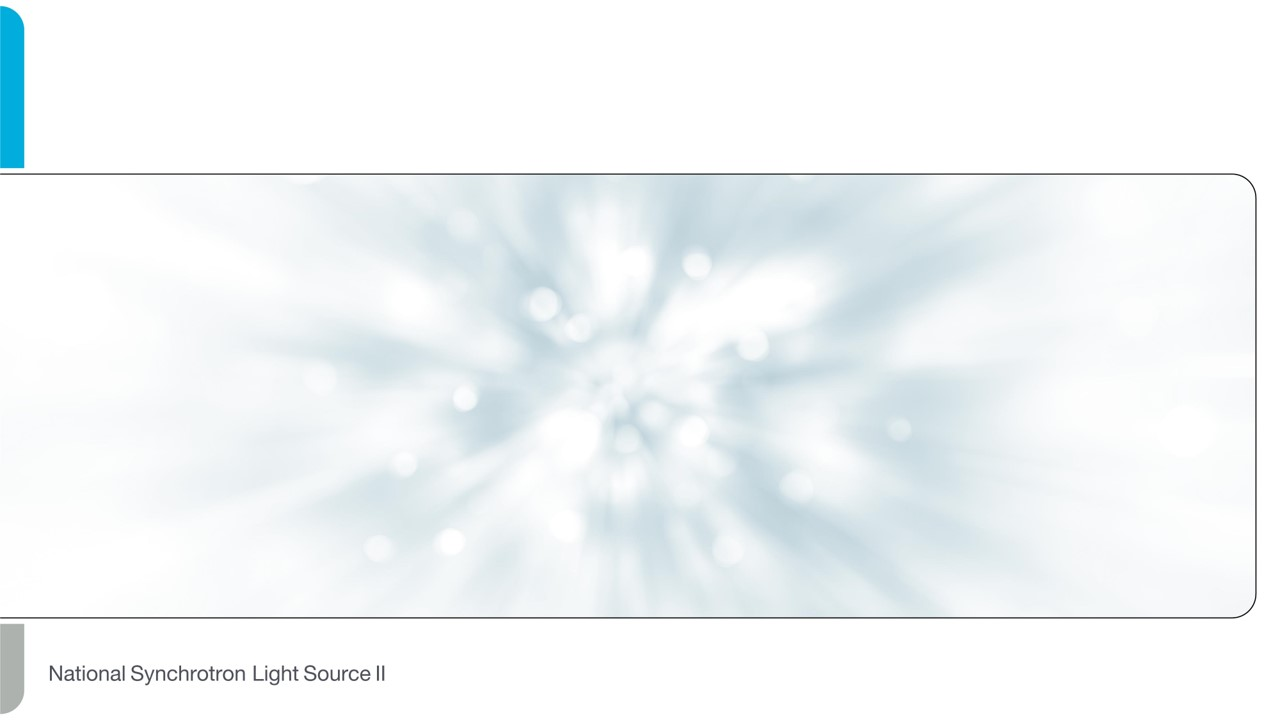
\includegraphics[width=\paperwidth,height=\paperheight]{assets/NSLS2_Divider.jpg}
    }
}

% ---------- Image placeholder command ----------
\newcommand{\imgplaceholder}[2][0.6]{%
    \begin{center}
        \fbox{\begin{minipage}{#1\textwidth}
            \centering\vspace{1.5cm}
            \textit{[Image: #2]}
            \vspace{1.5cm}
        \end{minipage}}
    \end{center}
}

% ---------- Title information ----------
\title{Bluesky QueueServer V2}
\author{Thomas Hopkins}
\institute{NSLS-II, Brookhaven National Laboratory}
\date{\today}

\begin{document}

% ==========================================================
% TITLE SLIDE
% ==========================================================
\titlebackground
\begin{frame}[plain]
    \titlepage
\end{frame}

% Switch background for remaining slides
\normalbackground

% ==========================================================
% FRAMING
% ==========================================================

\begin{frame}{What this talk is}
    \begin{columns}[T]
        \begin{column}{0.52\textwidth}
            \footnotesize
            \textbf{What I did}
            \begin{itemize}
                \item Wrote a second-generation queue server next to \legacy{}:
                      \code{bluesky\_queueserver.v2}
                \item Kept the shape already designed: one controller, one Bluesky worker process,
                      an editable persistent queue
                \item Changed the \emph{contracts}: identity, operation surface, concurrency,
                      failure handling, recovery
            \end{itemize}
            \vspace{0.3cm}
            \textbf{What I am asking for today}
            \begin{itemize}
                \item Agreement, or disagreement, on a short list of properties
                      I think \emph{any} Bluesky queue server needs
                \item Technical review of \vtwo{} as a candidate for the next major version
                \item Not a decision. Nothing shown here is ready to use in production yet.
            \end{itemize}
        \end{column}
        \begin{column}{0.44\textwidth}
            \begin{block}{Ground rules I set for myself}
                \footnotesize
                \begin{itemize}
                    \item Compare mechanisms. Every \legacy{} statement
                          cites a file and line in \code{manager/}, \code{bluesky-httpserver} or
                          \code{bluesky-queueserver-api}.
                    \item Where \legacy{} already does the right thing, say so.
                    \item Where \vtwo{} is incomplete, say so.
                    \item Everything in the demo runs against \code{ophyd.sim} only.
                \end{itemize}
            \end{block}
            \vspace{0.2cm}
            {\small\color{qsgray} Agenda: what 0.x got right $\rightarrow$ observations $\rightarrow$
            eight properties $\rightarrow$ what they mean once the service faces the internet $\rightarrow$
            architecture $\rightarrow$ live demo $\rightarrow$ status, costs, open questions.
            A glossary and a 0.x\,$\rightarrow$\,V2 phrasebook are in the backup slides.\par}
        \end{column}
    \end{columns}
\end{frame}

\begin{frame}{What \legacy{} got right -- and \vtwo{} keeps}
    \begin{columns}[T]
        \begin{column}{0.5\textwidth}
            \begin{exampleblock}{Core ideas}
                \footnotesize
                \begin{itemize}
                    \item \textbf{Manager / worker split.} Bluesky and Ophyd run in a separate process
                          from the thing that owns the queue.
                          \src{start\_manager.py:52-61}
                    \item \textbf{A persistent, editable queue.} Add, replace, move, remove;
                          survives a manager restart.
                          \src{plan\_queue\_ops.py:85-96}
                    \item \textbf{Worker environment from startup scripts} loaded in lexical order,
                          exactly like an IPython profile.
                    \item \textbf{Permissions as a concept}: not every user should reach every plan or device.
                    \item \textbf{Plan annotations and item validation} before execution.
                    \item \textbf{An HTTP edge with real authentication} (API keys, OIDC, LDAP, PAM, \ldots)
                          in \code{bluesky-httpserver}.
                \end{itemize}
            \end{exampleblock}
        \end{column}
        \begin{column}{0.46\textwidth}
            \footnotesize
            \textbf{What \vtwo{} carries forward}
            \begin{itemize}
                \item Controller $\neq$ worker; the worker owns the RunEngine and devices
                \item Durable queue, editable while running
                \item Profile-style startup directory, lexical order, IPython shell
                \item Scope-based authorization at the public edge
                \item Validation before anything is persisted
            \end{itemize}
            \vspace{0.2cm}
            \textbf{What \vtwo{} changes}
            \begin{itemize}
                \item \emph{Where} identity is established and \emph{who} trusts it
                \item \emph{What} a client may ask for
                \item \emph{How} the queue, the scheduler and the audit trail agree
                \item \emph{What happens} when the outcome of a plan cannot be proven
            \end{itemize}
            \vspace{0.15cm}
            {\color{qsgray} Years of beamline mileage went into 0.x. \vtwo{} tries to write down what
            that mileage taught us as contracts the code enforces.}
        \end{column}
    \end{columns}
\end{frame}

\begin{frame}{Observations that led to a rewrite rather than a patch}
    \small
    \begin{enumerate}
        \item \textbf{Identity is a request field.} The manager contract is \code{\{method, params\}};
              \code{user} and \code{user\_group} are supplied by the client and only checked for
              existence of the group. \src{manager.py:3759-3770, 2209-2222}
              The HTTP server fills them in from a real principal \src{routers/core\_api.py:201-212},
              but any 0MQ client fills them in itself. \src{qserver\_cli.py:49-50}
        \item \textbf{The public API is the worker namespace.} Plan names and dotted device paths
              resolve by \code{getattr} \src{profile\_ops.py:785-830, 993-1048};
              \code{function\_execute} calls allowed callables; \code{script\_upload} executes a
              client-supplied string in the worker. \src{worker.py:815-889}
              Allow/deny lists narrow the surface, but the surface \emph{is} the namespace.
        \item \textbf{Locks are strings, not principals.} \code{lock\_key} is chosen by the client;
              \code{unlock} accepts only the key. \src{manager.py:3458-3490, 3560-3575}
        \item \textbf{No concurrency contract on the queue.} \code{plan\_queue\_uid} is documented as
              informational; mutating calls take no expected version; last write wins.
              \src{plan\_queue\_ops.py:140-148}
        \item \textbf{Failure is rounded to ``retry''.} A failed, aborted or halted plan is pushed back to
              the \emph{front} of the queue with a new UID. \src{plan\_queue\_ops.py:1823-1859}
              A hard worker death has no recorded outcome path I could find. \src{manager.py:741-760, 1544-1550}
        \item \textbf{Clients poll.} Status every 1\,s, then reload queue/history when UIDs change.
              \src{api\_threads.py:66-149, 468-488; \_defaults.py:1-23}
        \item \textbf{Three repositories, unpinned against each other.}
              \src{bluesky-httpserver/pyproject.toml:16-19, bluesky-queueserver-api/pyproject.toml:16-19}
    \end{enumerate}
    \vspace{0.1cm}
    {\color{qsgray} Each of these is fixable in isolation. Together they are the design; changing them
    changes every public contract, which is why I think the honest shape is a major version, not a patch series.}
\end{frame}

% ==========================================================
% EIGHT PROPERTIES
% ==========================================================

\divider{Eight properties}{that I believe any Bluesky queue server needs, whichever codebase provides them}

% ----------------------------------------------------------
\begin{frame}{1 \quad Identity is established by the server; rights are scopes}
    {\footnotesize\itshape Why: the actor on an audit record must be something the server proved, not something
    the client typed. Staff, users and autonomous agents need different rights.}
    \vspace{0.05cm}
    \begin{columns}[T]
        \begin{column}{0.49\textwidth}
            \begin{alertblock}{\legacy{} today}
                \footnotesize
                \begin{itemize}
                    \item \code{bluesky-httpserver} does this well at the HTTP edge: API keys, access/refresh
                          tokens, OIDC/LDAP/PAM/SAML, roles $\rightarrow$ scopes such as
                          \code{write:queue:edit}. \src{authentication.py:259-307; core\_api.py:189-221}
                    \item It then forwards \code{\{"user": name, "user\_group": group\}} as plain fields
                          over 0MQ. \src{core\_api.py:201-212}
                    \item The manager trusts those fields; it checks only that the group exists.
                          \src{manager.py:2209-2222}
                    \item 0MQ CURVE uses one fixed client key pair, so the transport does not identify callers either.
                          \src{comms.py:18-19; manager\_config.rst:34-38}
                \end{itemize}
            \end{alertblock}
        \end{column}
        \begin{column}{0.49\textwidth}
            \begin{block}{\vtwo{}}
                \footnotesize
                \begin{itemize}
                    \item One process owns the public boundary; there is no second, unauthenticated control path.
                    \item OIDC bearer JWT, RS256, issuer/audience/JWKS verified; the principal is the \code{sub} claim.
                          \src{v2/auth.py:52-92}
                    \item Three fixed scopes: \code{queueserver:read} $\subset$ \code{control} $\subset$ \code{admin}.
                    \item Every durable mutation stores that principal; a body that tries to name an actor is rejected (422).
                    \item Only \code{/health} and \code{/ready} are unauthenticated, and they expose no principals or PIDs.
                \end{itemize}
            \end{block}
        \end{column}
    \end{columns}
    \vspace{0.1cm}
    {\footnotesize\color{qsgray} Demo: \code{qsv2 --as forged queue} $\rightarrow$ 401;\quad
    \code{qsv2 --as viewer submit} $\rightarrow$ 403 \code{scope 'queueserver:control' is required}.\par}
\end{frame}

% ----------------------------------------------------------
\begin{frame}{2 \quad A closed, versioned operation catalog, not a namespace}
    {\footnotesize\itshape Why: the remote contract should be reviewable without reading the worker's globals,
    and a change in meaning should be a visible version change.}
    \vspace{0.05cm}
    \begin{columns}[T]
        \begin{column}{0.49\textwidth}
            \begin{alertblock}{\legacy{} today}
                \footnotesize
                \begin{itemize}
                    \item A queue item is \code{\{"name": plan, "args", "kwargs"\}}; the worker resolves
                          the name and converts strings such as \code{"det.a"} by repeated \code{getattr}.
                          \src{profile\_ops.py:785-830, 993-1048}
                    \item \code{function\_execute} runs any allowed callable;
                          \code{script\_upload} \code{exec}s a client string in the namespace.
                          \src{manager.py:2954-3037; worker.py:815-889}
                    \item \code{existing\_plans\_and\_devices.yaml} + \code{user\_group\_permissions.yaml}
                          (regex allow/deny) narrow what is reachable. \src{profile\_ops.py:3736-3852}
                    \item Annotations give parameter types, but semantics are whatever the plan does today.
                \end{itemize}
            \end{alertblock}
        \end{column}
        \begin{column}{0.49\textwidth}
            \begin{block}{\vtwo{}}
                \footnotesize
                \begin{itemize}
                    \item A submission is \code{(operation\_id, operation\_version, parameters)}.
                    \item The worker publishes descriptors at startup: request and result JSON Schema,
                          required scope, orphan policy. \src{v2/contracts.py:195-224}
                    \item Controller and worker both validate; anything not in the catalog is refused
                          before persistence.
                    \item \code{worker\_revision} = SHA-256 over package, protocol, descriptors, Bluesky/Ophyd
                          versions, environment lock, startup and adapter sources. \src{v2/worker/sdk.py:192-207}
                    \item No plan names, no object paths, no scripts, no \code{execute\_plan}.
                \end{itemize}
            \end{block}
        \end{column}
    \end{columns}
    \vspace{0.1cm}
    {\footnotesize\color{qsgray} Demo: \code{num: 11} $\rightarrow$ 422 with the schema path;\quad
    \code{operation\_id: execute\_plan} $\rightarrow$ 422 \code{not in the worker catalog}.\par}
\end{frame}

% ----------------------------------------------------------
\begin{frame}{3 \quad Control is a lease on an identity; scheduling is separate authority}
    {\footnotesize\itshape Why: ``who may change the queue right now'' must be unambiguous, and a closed laptop
    must not end an overnight batch.}
    \vspace{0.05cm}
    \begin{columns}[T]
        \begin{column}{0.49\textwidth}
            \begin{alertblock}{\legacy{} today}
                \footnotesize
                \begin{itemize}
                    \item \code{lock} stores a client-chosen \code{lock\_key} plus a \code{user} string;
                          any caller presenting the key may act. \src{manager.py:3458-3490}
                    \item \code{unlock} takes only the key; the emergency key is a deployment secret.
                          \src{manager.py:3560-3575}
                    \item \code{queue\_start} flips manager state; \code{queue\_autostart} loops every 1\,s
                          while the queue is non-empty. \src{manager.py:1256-1282}
                    \item The manager keeps running the queue without a client -- the right behaviour,
                          and \vtwo{} keeps it.
                \end{itemize}
            \end{alertblock}
        \end{column}
        \begin{column}{0.49\textwidth}
            \begin{block}{\vtwo{}}
                \footnotesize
                \begin{itemize}
                    \item A \textbf{control lease}: one authenticated principal, TTL 5\,s--1\,h,
                          renew/release, admin override with a recorded reason.
                    \item Submitting, cancelling, replacing, reordering, start/stop and recovery
                          all require \emph{your} active lease.
                    \item Starting a \textbf{queue execution} durably records initiator, policy and the
                          admitted operations. That record, not the lease, authorizes the scheduler.
                    \item Admitted work continues after disconnect or lease expiry; lease expiry only
                          blocks \emph{new} external edits. \src{tests/v2/test\_scheduler.py:429-540}
                    \item Pending work is editable; claimed and running work is immutable.
                \end{itemize}
            \end{block}
        \end{column}
    \end{columns}
    \vspace{0.1cm}
    {\footnotesize\color{qsgray} Demo: \code{qsv2 --as admin submit} while \code{operator} holds the lease $\rightarrow$ 403
    \code{control lease belongs to another principal}.\par}
\end{frame}

% ----------------------------------------------------------
\begin{frame}{4 \quad Optimistic concurrency on the queue}
    {\footnotesize\itshape Why: a GUI, an agent and the scheduler all edit the same queue. ``Move item 3 up''
    must fail if the queue changed underneath you.}
    \vspace{0.05cm}
    \begin{columns}[T]
        \begin{column}{0.49\textwidth}
            \begin{alertblock}{\legacy{} today}
                \footnotesize
                \begin{itemize}
                    \item \code{plan\_queue\_uid} and \code{plan\_history\_uid} change on every mutation and
                          let clients avoid reloading.
                    \item They are documented as monitoring aids that ``may not represent a valid queue
                          state''. \src{plan\_queue\_ops.py:140-148}
                    \item \code{queue\_item\_add/update/move/remove} take no expected version;
                          the last writer wins. \src{manager.py:2379, 2476, 2553}
                    \item Every add assigns a fresh \code{item\_uid}, so an item has no stable identity
                          across a failed run. \src{manager.py:2390-2394}
                \end{itemize}
            \end{alertblock}
        \end{column}
        \begin{column}{0.49\textwidth}
            \begin{block}{\vtwo{}}
                \footnotesize
                \begin{itemize}
                    \item One monotonic \code{queue\_revision}; every queue response carries
                          \code{ETag: "qrev-N"}.
                    \item Every queue mutation requires \code{If-Match}: 428 if missing, 412 with the
                          current ETag if stale, no partial write.
                    \item Scheduler claims, completions and edits bump the \emph{same} revision in the same
                          SQLite transaction, so an edit racing a claim loses deterministically.
                          \src{v2/storage.py:2921-2946}
                    \item An operation keeps one UID from submission to terminal state; a replacement is a
                          new UID linked by \code{replaced\_by}.
                \end{itemize}
            \end{block}
        \end{column}
    \end{columns}
    \vspace{0.1cm}
    {\footnotesize\color{qsgray} Demo: \code{qsv2 --stale submit} $\rightarrow$ 412
    \code{queue revision 0 is stale; current revision is 2}, \code{ETag: "qrev-2"}.\par}
\end{frame}

% ----------------------------------------------------------
\begin{frame}{5 \quad Durable transactional state, an append-only audit log, push not poll}
    {\footnotesize\itshape Why: after a restart you must be able to say exactly what happened, in what order,
    and who asked for it. Clients should not have to guess by polling.}
    \vspace{0.05cm}
    \begin{columns}[T]
        \begin{column}{0.49\textwidth}
            \begin{alertblock}{\legacy{} today}
                \footnotesize
                \begin{itemize}
                    \item Redis lists and strings: \code{plan\_queue}, \code{running\_plan},
                          \code{plan\_history}, \code{plan\_queue\_mode}, \code{lock\_info}, \ldots{}
                          Survives a manager restart. \src{plan\_queue\_ops.py:85-96}
                    \item History holds each completed item with its result; there is no per-mutation
                          record of \emph{who} changed the queue.
                    \item Status is polled (default 1\,s); console output streams over PUB/SUB and
                          websockets. \src{api\_threads.py:66-149; core\_api.py:1123-1289}
                    \item Multi-key updates are not transactional across keys.
                \end{itemize}
            \end{alertblock}
        \end{column}
        \begin{column}{0.49\textwidth}
            \begin{block}{\vtwo{}}
                \footnotesize
                \begin{itemize}
                    \item SQLite, WAL, \code{synchronous=FULL}, foreign keys, application id \code{QSV2},
                          local disk only (NFS/CIFS/SSHFS/\ldots{} refused). \src{v2/storage.py:38-56, 728-751}
                    \item One \code{BEGIN IMMEDIATE} transaction writes the domain change, the revision,
                          the actor and an event. \src{v2/storage.py:3062-3088}
                    \item Events have monotonic ids: \code{GET /events?after=N} and SSE with
                          \code{Last-Event-ID} resume without gaps; 15\,s heartbeat comment.
                    \item Controller events and Bluesky documents are separate planes; the controller keeps
                          only run UIDs for correlation.
                    \item Schema migrations, backup with manifest, verified restore, admin CLI.
                \end{itemize}
            \end{block}
        \end{column}
    \end{columns}
    \vspace{0.1cm}
    {\footnotesize\color{qsgray} Demo: \code{qsv2 stream} shows every transition with actor and revision;
    restart the controller and replay from \code{after=0}.\par}
\end{frame}

% ----------------------------------------------------------
\begin{frame}{6 \quad Fail closed when an outcome cannot be proven}
    {\footnotesize\itshape Why: at a beamline, ``I do not know what the hardware did'' must never be rounded to
    ``failed, try again''.}
    \vspace{0.05cm}
    \begin{columns}[T]
        \begin{column}{0.49\textwidth}
            \begin{alertblock}{\legacy{} today}
                \footnotesize
                \begin{itemize}
                    \item A plan exception yields a \code{failed} report with run UIDs.
                          \src{worker.py:357-389}
                    \item Failed, aborted and halted items are appended to history \emph{and pushed back to the
                          front of the queue} with a new UID. \src{plan\_queue\_ops.py:1823-1859}
                    \item \code{ignore\_failures} mode continues to the next item. \src{manager.py:831-845}
                    \item \code{environment\_destroy} records the running item as failed.
                          \src{manager.py:657-686}
                    \item On a hard worker death the status poll returns \code{None} and only the
                          \code{ws is not None} branch is handled. \src{manager.py:741-760, 1544-1550}
                          I could not find a path that records the outcome.
                \end{itemize}
            \end{alertblock}
        \end{column}
        \begin{column}{0.49\textwidth}
            \begin{block}{\vtwo{}}
                \footnotesize
                \begin{itemize}
                    \item A claim writes a durable \textbf{attempt} (operation, worker instance, message id,
                          actor, revision, event) \emph{before} the worker is contacted.
                          \src{v2/controller.py:757-803}
                    \item Timeout, EOF, process exit, malformed frame, wrong correlation, invalid result
                          $\rightarrow$ \code{unknown}. Shutdown mid-attempt $\rightarrow$ \code{interrupted}.
                          Worker: RunEngine not idle or cleanup incomplete $\rightarrow$ \code{unknown}.
                          \src{v2/worker/runtime.py:391-430}
                    \item Any non-success blocks dispatch and stops the queue execution. Nothing is retried,
                          requeued or inferred. \src{tests/v2/test\_scheduler.py:549-604}
                    \item Retries never overwrite earlier evidence: a new attempt is a new row.
                \end{itemize}
            \end{block}
        \end{column}
    \end{columns}
    \vspace{0.1cm}
    {\footnotesize\color{qsgray} Demo: \code{qsv2 kill-worker} mid-plan $\rightarrow$ \code{operation.unknown}
    \code{\{cleanup\_completed: false\}}, \code{dispatch.blocked}, \code{/ready} $\rightarrow$ 503.\par}
\end{frame}

% ----------------------------------------------------------
\begin{frame}{7 \quad Explicit recovery, fenced worker authority}
    {\footnotesize\itshape Why: two processes must never both believe they own the RunEngine. Recovery is a human
    decision and should leave a record.}
    \vspace{0.05cm}
    \begin{columns}[T]
        \begin{column}{0.49\textwidth}
            \begin{alertblock}{\legacy{} today}
                \footnotesize
                \begin{itemize}
                    \item Watchdog restarts the manager after a 5--15\,s heartbeat gap.
                          \src{start\_manager.py:69, 217-221}
                    \item The new manager asks the watchdog if the worker is alive and
                          \emph{reconstructs} state from the worker's report: executing, paused, or
                          \code{exit\_status="unknown"}. \src{manager.py:3882-3928, 3948-3956}
                    \item Powerful and convenient; also the point where two views of the truth are
                          reconciled by inference, with no operator in the loop.
                    \item Worker restart is an API call (\code{environment\_open}) available to any
                          caller with the right scope.
                \end{itemize}
            \end{alertblock}
        \end{column}
        \begin{column}{0.49\textwidth}
            \begin{block}{\vtwo{}}
                \footnotesize
                \begin{itemize}
                    \item Controller lock and worker lock: \code{flock}, owner and mode checked, no symlinks.
                          The worker holds its lock until RunEngine cleanup and exit.
                          \src{v2/controller.py:86-126; v2/worker/runtime.py:44-75, 139-175}
                    \item \code{unknown}/\code{interrupted} require \textbf{fence evidence}: a successful exclusive
                          lock probe, recorded as \code{worker.fenced}. A PID is not evidence.
                    \item Recovery is \code{POST /recovery/acknowledge} with lease, revision and a note;
                          it fails with \code{prior worker authority has not ended} until fenced.
                    \item No reattachment to a surviving worker. On controller loss the worker requests a
                          RunEngine pause and exits (\code{request-stop}). \src{v2/worker/runtime.py:214-239}
                    \item Remaining queued work is \emph{not} resumed; a new execution must be started.
                \end{itemize}
            \end{block}
        \end{column}
    \end{columns}
    \vspace{0.1cm}
    {\footnotesize\color{qsgray} Demo: \code{qsv2 ack --note "..."} $\rightarrow$ 200, \code{/ready} $\rightarrow$ 200,
    execution state \code{stopped}, next item still \code{queued}.\par}
\end{frame}

% ----------------------------------------------------------
\begin{frame}{8 \quad Idempotent mutations and honest readiness}
    {\footnotesize\itshape Why: a retried request over hutch Wi-Fi must not submit twice. A supervisor needs to know
    which component is not ready, not just that the port answers.}
    \vspace{0.05cm}
    \begin{columns}[T]
        \begin{column}{0.49\textwidth}
            \begin{alertblock}{\legacy{} today}
                \footnotesize
                \begin{itemize}
                    \item Each call is one 0MQ REQ/REP exchange; a client that times out and resends
                          \code{queue\_item\_add} adds twice.
                    \item \code{status} reports \code{manager\_state}, \code{worker\_environment\_exists},
                          \code{re\_state}, queue/history UIDs. \src{manager.py:410-448}
                          Rich, but every client interprets the combination itself.
                    \item Health of Redis, watchdog and the 0MQ socket are not distinguished at the API.
                \end{itemize}
            \end{alertblock}
        \end{column}
        \begin{column}{0.49\textwidth}
            \begin{block}{\vtwo{}}
                \footnotesize
                \begin{itemize}
                    \item \code{Idempotency-Key} is required on every mutation, scoped to
                          (principal, method, path). Exact replay returns the stored status, body and ETag;
                          same key with a different body $\rightarrow$ 409. \src{v2/storage.py:2862-2917}
                    \item \code{/health}: the process answers. \code{/ready}: 200 only when controller lock,
                          storage, worker, fencing and dispatch are all ready; otherwise 503 with those five
                          coarse fields and nothing else.
                    \item Every response carries \code{X-Request-ID}; every error is
                          \code{\{code, message, details, request\_id\}}.
                \end{itemize}
            \end{block}
        \end{column}
    \end{columns}
    \vspace{0.1cm}
    {\footnotesize\color{qsgray} Demo: \code{qsv2 --key demo-renew lease renew} twice $\rightarrow$ 200, 200 (same body);
    then with \code{--ttl 900} $\rightarrow$ 409 \code{idempotency\_conflict}.\par}
\end{frame}

% ==========================================================
% SECURITY WHEN THE DOOR FACES THE INTERNET
% ==========================================================

\divider{When the door faces the internet}{the same eight properties, read as a security posture}

% ----------------------------------------------------------
\begin{frame}{Threat model for an internet-facing queue server}
    \framesubtitle{Authentication is NSLS-II's and BNL's job. Everything after the token is ours.}
    \begin{columns}[T]
        \begin{column}{0.48\textwidth}
            \scriptsize
            \textbf{What is behind the door}
            \begin{itemize}
                \item Motors, shutters, detectors: physical actions on a live instrument
                \item Beamtime: a stopped or corrupted queue is lost shifts
                \item Data integrity and provenance of what was collected and why
                \item The identities of staff and users, and the facility network behind the host
            \end{itemize}
            \vspace{0.15cm}
            \textbf{Who is on the other side}
            \begin{itemize}
                \item Anyone on the internet, before authentication
                \item A real user with phished or leaked credentials, or a compromised laptop
                \item An authenticated user doing something they are not supposed to be able to do
                \item A compromised intermediate host (proxy, HTTP server) on the facility network
                \item Automation and agents holding long-lived credentials
            \end{itemize}
        \end{column}
        \begin{column}{0.5\textwidth}
            \begin{block}{What must therefore hold}
                \scriptsize
                \begin{enumerate}
                    \item \textbf{One door.} Every control path authenticates; no second path that trusts the network.
                    \item \textbf{Identity from the identity provider}, verified by the service, never minted by it,
                          never supplied in a request.
                    \item \textbf{Least privilege per action}, decided server-side.
                    \item \textbf{No path from a request to code execution.} The remotely reachable surface is
                          reviewable and finite.
                    \item \textbf{Replay- and retry-safe mutations.}
                    \item \textbf{Non-repudiable audit}: who, what, when, in order.
                    \item \textbf{Safe under loss}: disconnects, timeouts and crashes end in a known state, not a guess.
                    \item \textbf{Bounded blast radius}: compromise of one component does not hand over the instrument.
                \end{enumerate}
            \end{block}
            {\footnotesize\color{qsgray} These are properties 1--8 again, with an adversary instead of a bug.\par}
        \end{column}
    \end{columns}
\end{frame}

% ----------------------------------------------------------
\begin{frame}{\legacy{}, read from the code: designed for a trusted network}
    \framesubtitle{Reasonable assumptions on a hutch LAN behind a VPN; each becomes an exposure on the internet}
    \begin{columns}[T]
        \begin{column}{0.34\textwidth}
            \begin{exampleblock}{What is already strong}
                \scriptsize
                \begin{itemize}
                    \item \code{bluesky-httpserver} has a serious authentication stack: OIDC, proxied OIDC,
                          Entra, SAML, LDAP, PAM; hashed API keys; refresh sessions; device-code flow.
                          \src{authenticators.py; authentication.py:259-307}
                    \item 25 fine-grained scopes mapped from roles; principal $\to$ resource group for plan/device
                          allow-lists. \src{authorization/\_defaults.py}
                    \item Token secrets support rotation. \src{authentication.py: decode\_token}
                    \item Per-group plan and device allow/deny lists at the manager.
                          \src{profile\_ops.py:3736-3852}
                \end{itemize}
            \end{exampleblock}
        \end{column}
        \begin{column}{0.64\textwidth}
            \begin{alertblock}{Assumptions that do not survive exposure}
                \scriptsize
                \begin{itemize}
                    \item \textbf{Two doors.} The manager's 0MQ port accepts \code{\{method, params\}} with
                          \code{user}/\code{user\_group} asserted by the caller; identity is exactly as strong
                          as the network ACL on port 60615. \src{manager.py:3759-3770, 2209-2222}
                    \item \textbf{CURVE encrypts, it does not authenticate.} The client key pair is fixed and
                          public. \src{comms.py:18-19; manager\_config.rst:34-38}
                    \item \textbf{The HTTP server is a token issuer.} It mints HS256 access and refresh tokens
                          from secrets it holds; a leaked secret forges any identity with any scope.
                          \src{authentication.py:71, create\_access\_token}
                    \item \textbf{Code execution is a feature.} \code{write:scripts} runs arbitrary Python in the
                          worker; \code{write:execute} calls allowed functions and is in the \emph{default}
                          \code{user} role. \src{core\_api.py:824-855; \_defaults.py}
                    \item \textbf{Plan arguments are a dynamic surface.} Strings resolve to namespace objects by
                          attribute path; safety depends on every beamline's allow-lists. \src{profile\_ops.py:785-830}
                    \item \textbf{Authorization is opt-in per route.} \code{GET /plans/existing} has no principal
                          dependency and answers unauthenticated. \src{core\_api.py:740-743}
                    \item \textbf{Compromise of the HTTP host is compromise of the instrument}: the
                          manager behind it trusts whatever that host says.
                \end{itemize}
            \end{alertblock}
        \end{column}
    \end{columns}
\end{frame}

% ----------------------------------------------------------
\begin{frame}{\vtwo{} posture, and what it does \emph{not} protect against}
    \begin{columns}[T]
        \begin{column}{0.5\textwidth}
            \begin{block}{Enforced today}
                \scriptsize
                \begin{itemize}
                    \item \textbf{One door.} HTTPS only; TLS files required at startup. No 0MQ, no second
                          control path; the worker is reachable only through a socketpair FD it inherits.
                    \item \textbf{No signing secret on the server.} Tokens are verified against the identity
                          provider's JWKS (RS256; \code{iss}, \code{aud}, \code{exp}, \code{iat}, \code{nbf}; 30\,s skew).
                          The controller cannot mint an identity. \src{v2/auth.py:52-92}
                    \item \textbf{Principal from the token only.} Bodies naming an actor are rejected.
                    \item \textbf{No request $\to$ code path.} No names, object paths, scripts or functions;
                          closed schemas (\code{additionalProperties: false}) validated on both sides. The tests
                          assert no \code{zmq}/\code{script}/\code{function}/\code{namespace}/\code{plan} route
                          exists. \src{tests/v2/test\_web\_api.py:284-288}
                    \item \textbf{Mutations need lease + revision + \code{Idempotency-Key}}; replays safe, conflicts 409.
                    \item \textbf{Audit:} every mutation records the principal; every response carries
                          \code{X-Request-ID}; events are append-only.
                    \item \textbf{No remote deployment levers:} no environment open/update/destroy, no package
                          or profile changes via the API; worker command from config, launched without a shell.
                    \item Lock files are \code{0600} and owner/mode checked; database on a local filesystem only;
                          \code{/health} and \code{/ready} expose no principals, PIDs or paths.
                \end{itemize}
            \end{block}
        \end{column}
        \begin{column}{0.48\textwidth}
            \begin{alertblock}{Not addressed; needs deployment or future work}
                \scriptsize
                \begin{itemize}
                    \item \textbf{No token revocation.} A bearer token is valid until \code{exp}. Mitigation:
                          short IdP token lifetimes; the lease TTL bounds mutation and SSE closes at expiry.
                    \item \textbf{No rate limiting or DoS protection.} Put a reverse proxy / WAF in front;
                          the controller is one asyncio process.
                    \item \textbf{The worker is not a sandbox.} Same OS user as the controller; profile and
                          adapter code are fully trusted. Containment is an OS/deployment matter.
                    \item \textbf{Authorization is per operation, not per experiment.} Any \code{control}
                          holder may run any catalogued operation; no proposal or resource-group model yet.
                    \item \textbf{Per-route authorization is still opt-in} in FastAPI; a missed dependency
                          would be the same class of bug as \code{/plans/existing}. Tests and review guard it.
                    \item \textbf{Identity-provider dependency.} JWKS is fetched and cached; an IdP outage blocks
                          new authentication (admitted work continues).
                    \item \textbf{Not yet reviewed by anyone but me.} A facility security review is needed.
                \end{itemize}
            \end{alertblock}
        \end{column}
    \end{columns}
\end{frame}

% ----------------------------------------------------------
\begin{frame}{Deployment shape for exposure}
    \begin{columns}[T]
        \begin{column}{0.56\textwidth}
            \begin{center}
            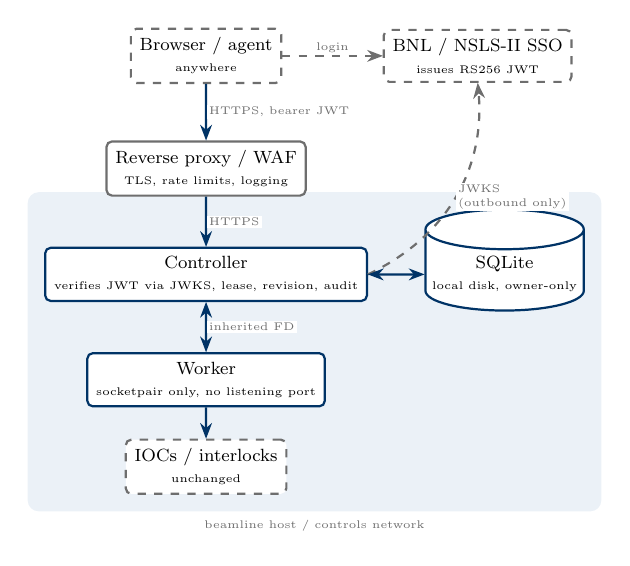
\begin{tikzpicture}[node distance=0.5cm and 0.6cm, scale=0.8, transform shape]
                \node[ext] (user) {Browser / agent\\\tiny anywhere};
                \node[ext, right=1.6cm of user] (idp) {BNL / NSLS-II SSO\\\tiny issues RS256 JWT};
                \node[box, below=0.9cm of user, draw=qsgray] (proxy) {Reverse proxy / WAF\\\tiny TLS, rate limits, logging};
                \node[box, below=0.8cm of proxy] (ctl) {Controller\\\tiny verifies JWT via JWKS, lease, revision, audit};
                \node[store, right=0.9cm of ctl] (db) {SQLite\\\tiny local disk, owner-only};
                \node[box, below=0.8cm of ctl] (wrk) {Worker\\\tiny socketpair only, no listening port};
                \node[ext, below=0.5cm of wrk] (ioc) {IOCs / interlocks\\\tiny unchanged};
                \draw[arrow, dashed, qsgray] (user) -- node[lbl, above] {login} (idp);
                \draw[arrow, dashed, qsgray] (ctl.east) to[bend right=35] node[lbl, right, align=left] {JWKS\\(outbound only)} (idp.south);
                \draw[arrow] (user) -- node[lbl, right] {HTTPS, bearer JWT} (proxy);
                \draw[arrow] (proxy) -- node[lbl, right] {HTTPS} (ctl);
                \draw[both, qsnavy] (ctl) -- (db);
                \draw[both, qsnavy] (ctl) -- node[lbl, right] {inherited FD} (wrk);
                \draw[arrow] (wrk) -- (ioc);
                \begin{scope}[on background layer]
                    \node[fill=qslight, rounded corners=4pt, fit=(ctl)(db)(wrk)(ioc), inner sep=6pt, label={[font=\tiny, text=qsgray]below:beamline host / controls network}] {};
                \end{scope}
            \end{tikzpicture}
            \end{center}
        \end{column}
        \begin{column}{0.42\textwidth}
            \footnotesize
            \textbf{What the picture buys}
            \begin{itemize}
                \item Exactly one inbound port on the beamline host: the controller's HTTPS.
                \item The host holds no identity-issuing secret; stealing the box does not forge users.
                \item Compromising the proxy yields HTTP requests that still need a valid JWT, a lease and the
                      current revision, and can still reach only catalogued operations.
                \item The worker has no network surface; its authority is bounded by the reviewed catalog
                      and ends with its lock.
                \item Everything that happened is in one append-only table on one disk.
            \end{itemize}
            \vspace{0.05cm}
            \textbf{What it does not buy}
            \begin{itemize}
                \item Protection from a legitimately authorized user doing a legitimate but harmful operation.
                      That is what reviewed operations, bounded parameters and interlocks are for.
                \item Anything the IdP gets wrong.
            \end{itemize}
        \end{column}
    \end{columns}
\end{frame}

% ==========================================================
% ARCHITECTURE
% ==========================================================

\divider{How \vtwo{} is put together}{same shape, different contracts}

% ----------------------------------------------------------
\begin{frame}{Process and trust boundaries, side by side}
    \begin{columns}[T]
        \begin{column}{0.5\textwidth}
            \centering {\footnotesize\bfseries\color{qsamber} \legacy{} \quad (3 repositories)}\\[0.1cm]
            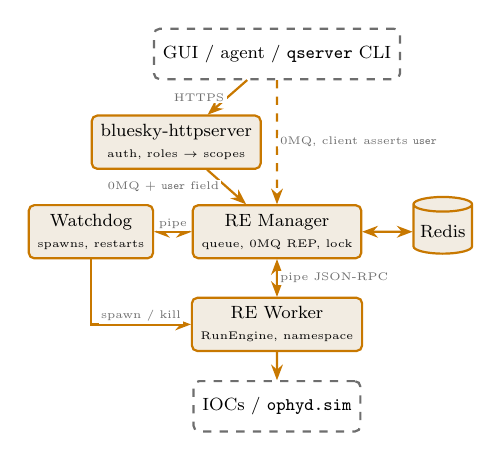
\begin{tikzpicture}[node distance=0.45cm and 0.5cm, scale=0.8, transform shape]
                \node[ext] (cli) {GUI / agent / \code{qserver} CLI};
                \node[legacybox, below=0.55cm of cli, xshift=-1.6cm] (http) {bluesky-httpserver\\\tiny auth, roles $\to$ scopes};
                \node[legacybox, below=0.55cm of http, xshift=1.6cm] (mgr) {RE Manager\\\tiny queue, 0MQ REP, lock};
                \node[legacystore, right=0.8cm of mgr] (redis) {Redis};
                \node[legacybox, left=0.6cm of mgr] (wd) {Watchdog\\\tiny spawns, restarts};
                \node[legacybox, below=0.6cm of mgr] (wrk) {RE Worker\\\tiny RunEngine, namespace};
                \node[ext, below=0.45cm of wrk] (ioc) {IOCs / \code{ophyd.sim}};
                \draw[legacyarrow] (cli) -- node[lbl, left] {HTTPS} (http);
                \draw[legacyarrow] (http) -- node[lbl, left, xshift=-2pt] {0MQ + \code{user} field} (mgr);
                \draw[legacyarrow, dashed] (cli) -- node[lbl, right] {0MQ, client asserts \code{user}} (mgr);
                \draw[both, qsamber] (mgr) -- (redis);
                \draw[both, qsamber] (wd) -- node[lbl, above] {pipe} (mgr);
                \draw[legacyarrow] (wd) |- node[lbl, pos=0.75, above] {spawn / kill} (wrk);
                \draw[both, qsamber] (mgr) -- node[lbl, right] {pipe JSON-RPC} (wrk);
                \draw[legacyarrow] (wrk) -- (ioc);
            \end{tikzpicture}
        \end{column}
        \begin{column}{0.5\textwidth}
            \centering {\footnotesize\bfseries\color{qsnavy} \vtwo{} \quad (1 repository, 1 release)}\\[0.1cm]
            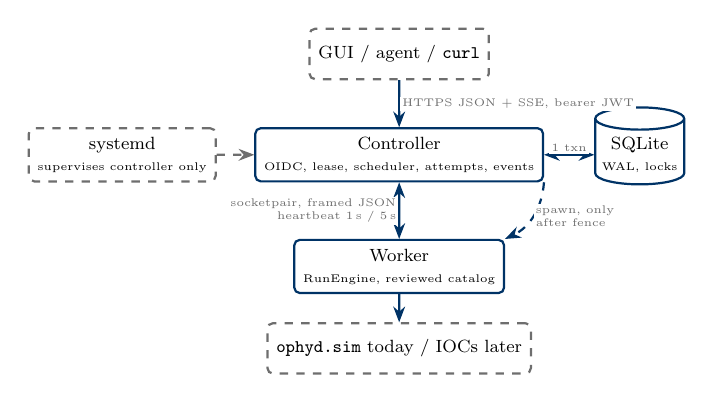
\begin{tikzpicture}[node distance=0.45cm and 0.5cm, scale=0.8, transform shape]
                \node[ext] (cli) {GUI / agent / \code{curl}};
                \node[box, below=0.75cm of cli] (ctl) {Controller\\\tiny OIDC, lease, scheduler, attempts, events};
                \node[store, right=0.8cm of ctl] (db) {SQLite\\\tiny WAL, locks};
                \node[ext, left=0.6cm of ctl] (sysd) {systemd\\\tiny supervises controller only};
                \node[box, below=0.9cm of ctl] (wrk) {Worker\\\tiny RunEngine, reviewed catalog};
                \node[ext, below=0.45cm of wrk] (ioc) {\code{ophyd.sim} today / IOCs later};
                \draw[arrow] (cli) -- node[lbl, right] {HTTPS JSON + SSE, bearer JWT} (ctl);
                \draw[both, qsnavy] (ctl) -- node[lbl, above] {1 txn} (db);
                \draw[arrow, dashed, qsgray] (sysd) -- (ctl);
                \draw[both, qsnavy] (ctl) -- node[lbl, left, align=right] {socketpair, framed JSON\\heartbeat 1\,s / 5\,s} (wrk);
                \draw[arrow] (wrk) -- (ioc);
                \draw[arrow, dashed] (ctl.south east) to[bend left=30] node[lbl, right, align=left] {spawn, only\\after fence} (wrk.north east);
            \end{tikzpicture}
        \end{column}
    \end{columns}
    \vspace{0.1cm}
    {\footnotesize\color{qsgray} Same split, same reason: keep Bluesky and Ophyd failures out of the process that
    owns the queue. \vtwo{} removes the second control path, the watchdog and the external store;
    the controller is the only durable authority.\par}
\end{frame}

% ----------------------------------------------------------
\begin{frame}{Operation lifecycle}
    \begin{center}
    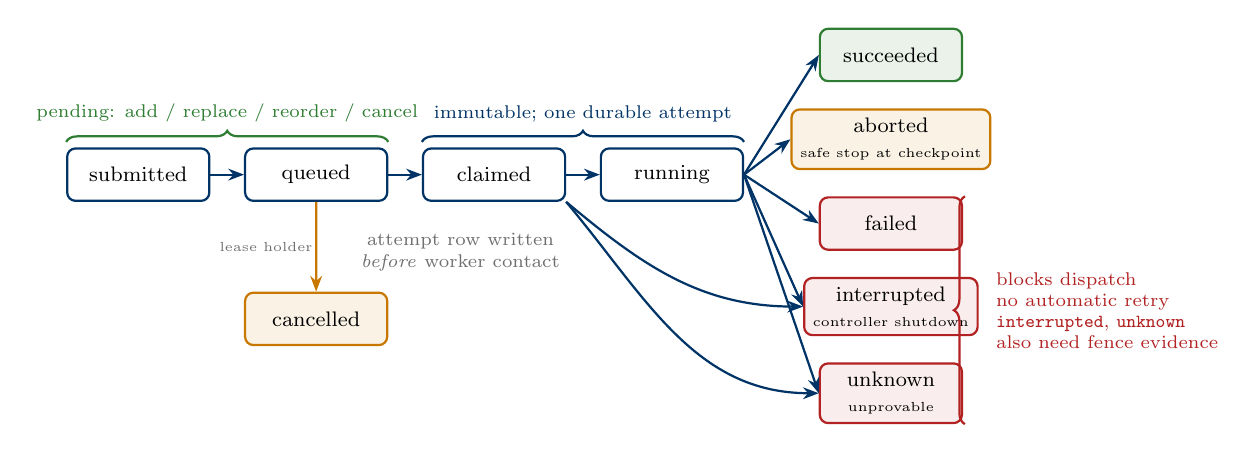
\begin{tikzpicture}[node distance=0.35cm and 0.45cm, scale=0.95, transform shape]
        \node[state] (sub) {submitted};
        \node[state, right=of sub] (que) {queued};
        \node[state, right=of que] (cla) {claimed};
        \node[state, right=of cla] (run) {running};
        \node[good, right=1.0cm of run, yshift=1.6cm] (ok) {succeeded};
        \node[stop, below=of ok] (abo) {aborted\\\tiny safe stop at checkpoint};
        \node[bad, below=of abo] (fail) {failed};
        \node[bad, below=of fail] (intr) {interrupted\\\tiny controller shutdown};
        \node[bad, below=of intr] (unk) {unknown\\\tiny unprovable};
        \node[stop, below=1.2cm of que] (can) {cancelled};
        \draw[arrow] (sub) -- (que);
        \draw[arrow] (que) -- (cla);
        \draw[arrow] (cla) -- (run);
        \foreach \t in {ok,abo,fail,intr,unk} { \draw[arrow] (run.east) -- (\t.west); }
        \draw[arrow] (cla.south east) to[out=-40, in=180] (intr.west);
        \draw[arrow] (cla.south east) to[out=-50, in=180] (unk.west);
        \draw[arrow, qsamber] (que) -- node[lbl, left] {lease holder} (can);
        \draw[decorate, decoration={brace, amplitude=4pt, raise=2pt}, qsgreen, thick]
            (sub.north west) -- (que.north east) node[midway, above=6pt, font=\scriptsize, text=qsgreen] {pending: add / replace / reorder / cancel};
        \draw[decorate, decoration={brace, amplitude=4pt, raise=2pt}, qsnavy, thick]
            (cla.north west) -- (run.north east) node[midway, above=6pt, font=\scriptsize, text=qsnavy] {immutable; one durable attempt};
        \node[font=\scriptsize, text=qsgray, below=0.3cm of cla, xshift=-0.45cm, align=center] {attempt row written\\\emph{before} worker contact};
        \draw[decorate, decoration={brace, amplitude=4pt, mirror, raise=2pt}, qsred, thick]
            ($(fail.north east)+(0.1,0)$) -- ($(unk.south east)+(0.1,0)$) node[midway, right=6pt, font=\scriptsize, text=qsred, align=left] {blocks dispatch\\no automatic retry\\\scriptsize\texttt{interrupted}, \texttt{unknown}\\also need fence evidence};
    \end{tikzpicture}
    \end{center}
    \vspace{-0.1cm}
    {\footnotesize A queue execution is \code{running} $\to$ \code{stopping} (stop after current) $\to$ \code{completed} $\mid$
    \code{stopped} $\mid$ \code{blocked}. Policy today: \code{stop\_on\_non\_success}.}
\end{frame}

% ----------------------------------------------------------
\begin{frame}{The private worker protocol}
    \begin{columns}[T]
        \begin{column}{0.55\textwidth}
            \footnotesize
            \begin{itemize}
                \item \textbf{Transport:} \code{socketpair(AF\_UNIX)} created by the controller; the child FD is passed
                      on the command line, never a TCP port or a shell. \src{v2/worker\_protocol.py:301-322}
                \item \textbf{Framing:} 4-byte length + JSON, 1\,MiB cap enforced before the body is read.
                \item \textbf{Correlation:} every message has \code{message\_id}; responses must carry the request's
                      \code{correlation\_id}, the attempt UID and the worker instance UID. A mismatch is \code{unknown},
                      not ``probably fine''.
                \item \textbf{Liveness during a plan:} the RunEngine runs in a one-thread executor; the asyncio
                      control loop keeps answering \code{ping} and \code{safe\_stop} on the same socket.
                      \src{v2/worker/runtime.py:211-246, 364-371}
                \item \textbf{Safe stop:} \code{RE.request\_pause(defer=True)}, acknowledged, cleanup awaited.
                \item \textbf{Orphan policy:} on controller loss the worker stops accepting work, requests the pause,
                      waits for cleanup, releases its lock and exits with code 2.
                \item \textbf{Worker lock} is the fence: acquired at start, released after executor shutdown.
            \end{itemize}
        \end{column}
        \begin{column}{0.43\textwidth}
            \begin{block}{Message types}
                \scriptsize
                \begin{tabular}{@{}l@{\hspace{6pt}}l@{}}
                    W $\to$ C & \code{startup.catalog}, \code{startup.ready} \\
                    C $\to$ W & \code{execution.request} \\
                    W $\to$ C & \code{execution.accepted}, \code{execution.completed} \\
                    both & \code{ping} / \code{pong} \\
                    C $\to$ W & \code{safe\_stop.request} $\to$ \code{.ack} \\
                    C $\to$ W & \code{shutdown.request} $\to$ \code{.ack} \\
                \end{tabular}
            \end{block}
            \begin{block}{Faults exercised by tests}
                \scriptsize
                \code{eof}, \code{exit}, \code{timeout}, \code{malformed}, \code{oversized}, \code{wrong-protocol},
                \code{wrong-worker}, \code{wrong-attempt}, \code{wrong-correlation}, \code{invalid-result},
                socket loss mid-plan, SIGKILL mid-plan. Each becomes exactly one \code{unknown} and one dispatch block.
                \src{tests/v2/fault\_worker.py; test\_worker\_runtime.py:488-560}
            \end{block}
        \end{column}
    \end{columns}
\end{frame}

% ----------------------------------------------------------
\begin{frame}[fragile]{Adopting a beamline without rewriting its profile collection}
    \begin{columns}[T]
        \begin{column}{0.42\textwidth}
            \footnotesize
            The worker's \emph{profile mode} loads the existing startup directory the way 0.x and IPython do:
            top-level \code{*.py}/\code{*.ipy} in lexical order, one isolated \code{InteractiveShell}.
            Then it runs one extra file, the \textbf{adapter}, and calls
            \code{register\_operations(registry, profile)}. \src{v2/worker/profile.py:31-81}
            \begin{itemize}
                \item \code{profile} is the loaded namespace, read-only.
                \item Device maps are explicit deployment code, not client input.
                \item Only the path reachable from a registered operation needs hardening;
                      commissioning helpers stay private.
                \item Startup and adapter hashes become part of \code{worker\_revision}.
                \item \code{existing\_plans\_and\_devices.yaml} and annotations are good \emph{offline} inputs
                      for drafting adapters; a human commits each one.
            \end{itemize}
        \end{column}
        \begin{column}{0.58\textwidth}
\begin{lstlisting}[style=python, aboveskip=0pt, belowskip=0pt, breaklines=false]
# adapter.py -- private worker code, reviewed and committed
DETECTORS = {"xs": xs, "merlin": merlin}
MOTORS = {"ssx": zpssx, "ssy": zpssy}

class Fly2DRequest(StrictModel):
    detectors: list[Literal["xs", "merlin"]]
    fast_axis: Literal["ssx", "ssy"]
    slow_axis: Literal["ssx", "ssy"]
    fast_range: tuple[float, float]
    slow_range: tuple[float, float]
    fast_points: Annotated[int, Field(ge=2, le=4000)]
    slow_points: Annotated[int, Field(ge=1, le=4000)]
    exposure: Annotated[float, Field(gt=0, le=10)]

def register_operations(registry, profile):
    @registry.register(
        operation_id="hxn.fly2d", operation_version="1",
        request_model=Fly2DRequest, result_model=RunUids,
        required_scope=AuthorizationScope.CONTROL,
        orphan_policy=OrphanPolicy.REQUEST_STOP)
    def prepare(request, context):
        fast, slow = MOTORS[request.fast_axis], MOTORS[request.slow_axis]
        plan = profile["fly2dpd"](
            [DETECTORS[d] for d in request.detectors],
            fast, *request.fast_range, request.fast_points,
            slow, *request.slow_range, request.slow_points,
            request.exposure)
        return PreparedOperation(
            plan=plan,
            build_result=lambda uids: RunUids(run_uids=list(uids)))
\end{lstlisting}
        \end{column}
    \end{columns}
\end{frame}

% ==========================================================
% COMPARISON AND DEMO
% ==========================================================

\begin{frame}{Side by side (1/2): boundary and contract}
    \footnotesize
    \renewcommand{\arraystretch}{1.35}
    \begin{tabular}{@{}L{2.7cm}L{5.4cm}L{5.4cm}@{}}
        \toprule
        & \textbf{\color{qsamber}\legacy{}} & \textbf{\color{qsnavy}\vtwo{}} \\
        \midrule
        Public transport & 0MQ REQ/REP (+ PUB/SUB console); REST via a second service & HTTPS JSON + SSE from the controller itself \\
        Identity & Authenticated at the HTTP server; \code{user}/\code{user\_group} fields trusted by the manager & OIDC JWT verified by the controller; principal = \code{sub} \\
        Authorization & Roles $\to$ fine-grained scopes (HTTP); group allow/deny lists (manager) & Three scopes; per-operation \code{required\_scope} in the catalog \\
        What a client can request & Any allowed plan/function name with args, device paths, scripts & Catalogued \code{(operation\_id, version)} with closed JSON Schema \\
        Exclusive control & String \code{lock\_key}, optional, not identity-bound & Lease: one principal, TTL, renew/release, audited override \\
        Queue concurrency & Informational \code{plan\_queue\_uid}; last write wins & \code{queue\_revision} + \code{If-Match}/ETag; 412 on stale \\
        Item identity & New \code{item\_uid} on every add and on push-back & One operation UID for life; attempts are separate rows \\
        Request retry safety & None at protocol level & Mandatory \code{Idempotency-Key}; 409 on conflicting reuse \\
        Readiness & \code{status} fields interpreted by each client & \code{/ready} 200/503 with five component fields \\
        \bottomrule
    \end{tabular}
\end{frame}

\begin{frame}{Side by side (2/2): state, failure, lifecycle}
    \footnotesize
    \renewcommand{\arraystretch}{1.35}
    \begin{tabular}{@{}L{2.7cm}L{5.4cm}L{5.4cm}@{}}
        \toprule
        & \textbf{\color{qsamber}\legacy{}} & \textbf{\color{qsnavy}\vtwo{}} \\
        \midrule
        State store & Redis lists/strings & SQLite WAL on local disk, one transaction per mutation \\
        Audit & Plan history with results & Append-only events with actor, revision, cursor; SSE resume \\
        Plan failure & Push back to queue front; optional ignore-failures & \code{failed} blocks dispatch; never requeued automatically \\
        Unprovable outcome & Depends on which poll noticed & \code{unknown}; dispatch blocked; fence + acknowledgement required \\
        Manager/controller restart & Watchdog restarts; manager reattaches to live worker & Fail closed; never reattaches; worker self-stops on controller loss \\
        Worker restart & \code{environment\_open/close/destroy} via API & Only the controller, only after the previous lock is provably released \\
        Stopping & pause/resume/stop/abort/halt, \code{queue\_stop} & Safe stop at next checkpoint; stop after current \\
        Packaging & 3 repos, mutually unpinned & 1 repo, 1 version; worker revision hashes environment lock \\
        Python & 3.10+ (httpserver, api) & 3.11+ (shared distribution) \\
        \bottomrule
    \end{tabular}
\end{frame}

\begin{frame}[fragile]{Live demo}
    \begin{columns}[T]
        \begin{column}{0.6\textwidth}
\begin{lstlisting}[style=http, basicstyle=\ttfamily\tiny, breaklines=false]
# terminal 1: controller (it spawns the worker)
pixi run -e py312 python demo/setup.py
pixi run -e py312 start-qserver-v2 --config demo/state/controller.yml --port 8443
# terminal 2: durable event stream
qsv2 stream
# terminal 3: the walk-through
qsv2 ready                              # 200, five components
qsv2 --as forged queue                  # 401 unknown signing key
qsv2 --as viewer submit                 # 403 scope required
qsv2 lease acquire --ttl 600            # 201 holder=operator
qsv2 --as admin submit                  # 403 lease belongs to another principal
qsv2 submit --raw '{... "num": 11}'     # 422 schema path
qsv2 submit --raw '{"operation_id": "execute_plan", ...}'   # 422 not in catalog
qsv2 submit --num 2 --delay 0.5         # 201 ETag "qrev-1"
qsv2 --stale submit                     # 412 current revision
qsv2 start                              # 201 admitted work recorded
qsv2 --key k lease renew  (twice)       # 200, 200 identical
qsv2 --key k lease renew --ttl 900      # 409 idempotency_conflict

qsv2 submit --num 10 --delay 2 && qsv2 start
qsv2 kill-worker                        # SIGKILL mid-plan
qsv2 ready                              # 503 dispatch=blocked
qsv2 ack --note "..."                   # 200; worker.fenced already recorded
qsv2 ready                              # 200; next item queued, not resumed
# restart terminal 1, then:
qsv2 events --after 0                   # everything is still there
\end{lstlisting}
        \end{column}
        \begin{column}{0.38\textwidth}
            \footnotesize
            \textbf{What to watch for}
            \begin{itemize}
                \item Every mutation prints its \code{If-Match} and \code{Idempotency-Key}; every response its ETag.
                \item Rejections happen \emph{before} any write: the revision does not move on 401/403/412/422.
                \item In the stream: \code{actor} is the principal for edits and \code{scheduler} for claims;
                      \code{qrev} increases monotonically.
                \item After \code{kill-worker}: \code{operation.unknown} carries
                      \code{cleanup\_completed: false} and the transport diagnostic;
                      \code{dispatch.blocked} carries \code{requires\_fence: true};
                      \code{worker.fenced} records the lock probe.
                \item Acknowledgement needs the lease, the current revision and a note. The remaining item is
                      \emph{not} resumed.
            \end{itemize}
            \vspace{0.2cm}
            {\color{qsgray}\footnotesize \code{qsv2} is \code{demo/qsv2.py}: ~200 lines of \code{httpx}, no SDK.
            \code{demo/walkthrough.sh} runs the same sequence with pauses.\par}
        \end{column}
    \end{columns}
\end{frame}

% ==========================================================
% STATUS, COSTS, PATH, DISCUSSION
% ==========================================================

\divider{Where \vtwo{} actually is}{what exists, what does not, what I chose not to build}

% ----------------------------------------------------------
\begin{frame}{Implemented today vs.\ not yet}
    \begin{columns}[T]
        \begin{column}{0.5\textwidth}
            \begin{exampleblock}{Runs today (simulator only)}
                \footnotesize
                \begin{itemize}
                    \item Controller: authority lock, scheduler, durable attempts, dispatch blocks, recovery
                    \item SQLite store: migrations, revisions, events, lease, idempotency records;
                          backup/restore/migrate via \code{qserver-v2-admin}
                    \item OIDC JWT authentication, three scopes, HTTPS + SSE, OpenAPI
                    \item Worker protocol: heartbeat, correlation, safe stop, orphan stop, lock and fencing
                    \item Worker SDK (\code{registry.register}), profile-mode loader, worker revision
                    \item One operation: \code{simulated-count} v1 on \code{ophyd.sim}; systemd unit, example configs
                    \item 81 behavioural tests in \code{tests/v2/} (contracts, storage, scheduler, recovery,
                          web, worker runtime, admin), including the fault matrix
                \end{itemize}
            \end{exampleblock}
        \end{column}
        \begin{column}{0.48\textwidth}
            \begin{alertblock}{Not yet}
                \footnotesize
                \begin{itemize}
                    \item Any real beamline adapter, test IOC run, or hardware approval
                    \item Operator UI, client SDK, console-output streaming
                    \item Pause/resume/stop/abort/halt as a user-facing surface; today only
                          \emph{safe stop at next checkpoint} and \emph{stop after current}
                    \item Loop mode, instructions, batch submission
                    \item Interactive kernel, script upload, function execution (deliberately; next slide)
                    \item Compatibility with \code{bluesky-queueserver-api}, \code{bluesky-widgets},
                          \code{bluesky-httpserver}
                    \item HA, PostgreSQL, SQLite over NFS, worker reattachment, automatic retry
                \end{itemize}
            \end{alertblock}
            \vspace{0.1cm}
            {\scriptsize\color{qsgray} Size, for orientation: \code{v2/} is about 7.3k lines;
            \code{manager/} about 20k; \code{bluesky-httpserver} and \code{bluesky-queueserver-api}
            roughly 6k each excluding docstrings. Smaller because it does less, on purpose.\par}
        \end{column}
    \end{columns}
\end{frame}

% ----------------------------------------------------------
\begin{frame}{Things I deliberately did not build}
    \small
    \renewcommand{\arraystretch}{1.15}
    \begin{tabular}{@{}L{4.2cm}L{9.0cm}@{}}
        \toprule
        \textbf{Not built} & \textbf{Why} \\
        \midrule
        A generic \code{execute\_plan(name, args, kwargs)} & It recreates the namespace-as-API surface. Everything else in \vtwo{} is downstream of refusing it. \\
        0.x protocol or queue compatibility & Compatibility keeps the dynamic execution, transport and storage contracts that are the reason for the rewrite. Coexistence instead: separate state, endpoints and authority. \\
        Controller-managed environment updates (install, git pull, env open/close) & Deployment changes belong to deployment tooling with their own audit; the worker revision records what ran. \\
        Watchdog and worker reattachment & Independent lifetimes are where the two views of the truth diverge. \vtwo{} fails closed and asks a human. \\
        Redis & SQLite gives the transaction, revision and event boundary one controller needs, on a local disk, with no second service. \\
        Bluesky inside the controller & It couples the public authority to beamline dependencies and plan failures. \\
        Active-active or HA controllers & Leadership and fencing across hosts is not justified for one instrument; one authority is the point. \\
        Bluesky document storage & Documents stay in the RunEngine subscriptions; the controller keeps run UIDs only. \\
        \bottomrule
    \end{tabular}
\end{frame}

% ----------------------------------------------------------
\begin{frame}{Costs and risks, honestly}
    \begin{columns}[T]
        \begin{column}{0.5\textwidth}
            \textbf{What beamlines pay}
            \small
            \begin{itemize}
                \item \textbf{Adapters are work.} Every exposed workflow needs a request model, a device map
                      and a reviewed registration. Boilerplate risk is real; offline generation from
                      \code{existing\_plans\_and\_devices.yaml} and annotations can draft them, not commit them.
                \item \textbf{Less freedom at the API.} No ad-hoc plan, no script upload, no function call
                      from a GUI. Interactive Bluesky stays available for that; it just does not share
                      authority with \vtwo{}.
                \item \textbf{An identity provider is required.} Today's single-user API key is not an option.
                \item \textbf{Local disk only.} The controller host owns the state; moving it is a backup/restore.
                \item \textbf{Operators see new words}: take control, release control, stop after current,
                      recovery required. The UI must hide lease IDs and revisions.
            \end{itemize}
        \end{column}
        \begin{column}{0.48\textwidth}
            \textbf{What the project pays}
            \small
            \begin{itemize}
                \item \textbf{Two codebases during transition.} 0.x needs a stated maintenance policy
                      while \vtwo{} matures; I do not think both should be developed indefinitely.
                \item \textbf{The ecosystem does not follow for free.} \code{bluesky-widgets},
                      \code{queue-monitor}, agents built on \code{bluesky-queueserver-api} need a \vtwo{} client.
                \item \textbf{My failure matrix may be wrong.} It is tested against a fault-injecting
                      worker and the simulator, not against years of beamline incidents. That knowledge is
                      in this room.
                \item \textbf{Single author so far.} Review by people who know why 0.x made each choice
                      is the fastest way to find what I missed.
            \end{itemize}
        \end{column}
    \end{columns}
\end{frame}

% ----------------------------------------------------------
\begin{frame}{A path, not a cliff}
    \begin{columns}[T]
        \begin{column}{0.5\textwidth}
            \small
            \begin{enumerate}
                \item \textbf{Agree on the properties first.} If the eight properties are right, they constrain
                      any implementation, including a hypothetical 0.x successor that is not \vtwo{}.
                \item \textbf{Review \vtwo{} against them.} Code, tests and the failure matrix are in-tree;
                      the simulator demo runs on a laptop.
                \item \textbf{One workflow, one beamline, simulation or test IOC.} Load the real profile in
                      profile mode, write one adapter, run the failure matrix against it.
                \item \textbf{Coexist.} 0.x keeps serving what has not moved. No shared queue, endpoint,
                      worker or state; one authority per instrument at a time.
                \item \textbf{Decide the 0.x policy together}: security fixes only, or feature freeze with a date.
                \item \textbf{Only then} talk about hardware, a UI, and a client library.
            \end{enumerate}
        \end{column}
        \begin{column}{0.48\textwidth}
            \begin{block}{What would change my mind}
                \small
                \begin{itemize}
                    \item A property on the list that you can show is wrong for beamline operations.
                    \item A workflow that cannot be expressed as a catalogued operation without losing
                          something scientifically essential.
                    \item Evidence that 0.x can be brought to these properties incrementally without breaking
                          its public API anyway.
                \end{itemize}
            \end{block}
            \vspace{0.2cm}
            {\small\color{qsgray} My preference is clear: converge on one implementation once \vtwo{} has
            earned it, rather than maintain two. I would rather be argued out of that in this room than
            discover the reason at a beamline.\par}
        \end{column}
    \end{columns}
\end{frame}

% ----------------------------------------------------------
\begin{frame}{Questions I would like this group to answer}
    \normalsize
    \begin{enumerate}
        \setlength{\itemsep}{0.25cm}
        \item Which of the eight properties do you disagree with, and why?
        \item Which 0.x capability did I drop that you would fight to keep
              (interactive kernel, script upload, function execution, loop mode, \ldots)?
        \item Is ``catalog, not namespace'' workable for the beamlines you support?
              Which workflow would you pilot first?
        \item Where is the failure matrix wrong? What incident would it have handled badly?
        \item We intend to expose this service on the internet behind facility SSO.
              Which of the 0.x assumptions on the security slide would you be comfortable keeping there?
        \item If \vtwo{} proceeds, what is the right maintenance policy for 0.x?
    \end{enumerate}
    \vspace{0.4cm}
    \begin{center}
        {\normalsize\color{qsgray} Code: \code{src/bluesky\_queueserver/v2/} \quad
        Tests: \code{src/bluesky\_queueserver/tests/v2/} \quad
        Docs: \code{docs/source/queueserver\_v2.rst} \quad
        Demo: \code{demo/}\\[0.2cm]
        \footnotesize Backup slides: the watchdog question, API surface, durable model, example payloads, glossary, 0.x\,$\rightarrow$\,V2 phrasebook.}
    \end{center}
\end{frame}

% ==========================================================
% BACKUP
% ==========================================================

\divider{Backup}{reference material}

% ----------------------------------------------------------
\begin{frame}{Backup: public HTTP surface}
    \footnotesize
    \begin{columns}[T]
        \begin{column}{0.46\textwidth}
            \textbf{Queries} (\code{queueserver:read})
            \begin{itemize}
                \item \code{GET /health}, \code{GET /ready} \hfill {\color{qsgray}unauthenticated}
                \item \code{GET /api/v2/openapi.json}
                \item \code{GET /api/v2/catalog}
                \item \code{GET /api/v2/control-lease}
                \item \code{GET /api/v2/queue} \hfill {\color{qsgray}ETag \code{"qrev-N"}}
                \item \code{GET /api/v2/queue-executions/\{uid\}}
                \item \code{GET /api/v2/operations/\{uid\}}
                \item \code{GET /api/v2/attempts/\{uid\}}
                \item \code{GET /api/v2/events?after=\&limit=}
                \item \code{GET /api/v2/events/stream} \hfill {\color{qsgray}SSE, \code{Last-Event-ID}}
            \end{itemize}
        \end{column}
        \begin{column}{0.52\textwidth}
            \textbf{Commands} (\code{queueserver:control}; all need \code{Idempotency-Key}; queue-changing ones need \code{If-Match})
            \begin{itemize}
                \item \code{POST /api/v2/control-lease} \code{/renew} \code{/release}
                \item \code{POST /api/v2/control-lease/override} \hfill {\color{qsgray}\code{admin}, reason}
                \item \code{POST /api/v2/operations}
                \item \code{PUT /api/v2/operations/\{uid\}} \hfill {\color{qsgray}replace pending}
                \item \code{DELETE /api/v2/operations/\{uid\}} \hfill {\color{qsgray}cancel pending}
                \item \code{POST /api/v2/queue/reorder} \hfill {\color{qsgray}complete permutation}
                \item \code{POST /api/v2/queue-executions}
                \item \code{POST /api/v2/queue-executions/\{uid\}/stop} \hfill {\color{qsgray}after current}
                \item \code{POST /api/v2/attempts/\{uid\}/safe-stop}
                \item \code{POST /api/v2/recovery/acknowledge}
            \end{itemize}
            \vspace{0.1cm}
            Errors: 401 \code{authentication\_failed}, 403 \code{forbidden}, 404 \code{not\_found},
            409 \code{state\_conflict}/\code{idempotency\_conflict}, 412 \code{stale\_revision},
            422 \code{validation\_error}/\code{invalid\_request}, 428 \code{precondition\_required},
            503 \code{unavailable}.
        \end{column}
    \end{columns}
\end{frame}

% ----------------------------------------------------------
\begin{frame}{Backup: durable model and event types}
    \footnotesize
    \begin{columns}[T]
        \begin{column}{0.5\textwidth}
            \textbf{SQLite tables} \src{v2/storage.py:396-552}
            \begin{itemize}
                \item \code{operations} -- immutable intent, state, result, \code{replaced\_by}
                \item \code{queue\_entries} -- pending order (\code{position} unique)
                \item \code{queue\_executions}, \code{queue\_execution\_admissions}
                \item \code{execution\_attempts} -- one row per controller-authorized invocation
                \item \code{worker\_instances} -- revision, provenance, catalog, lock path
                \item \code{dispatch\_blocks} -- kind, \code{requires\_fence}, fence/ack evidence
                \item \code{control\_lease} -- singleton: subject, expiry
                \item \code{controller\_metadata} -- singleton: \code{queue\_revision}, paths, active block
                \item \code{controller\_events} -- append-only, \code{event\_id} autoincrement
                \item \code{idempotency\_records} -- (principal, method, target, key) $\to$ stored response
                \item \code{schema\_migrations}
            \end{itemize}
        \end{column}
        \begin{column}{0.48\textwidth}
            \textbf{Event types} \src{v2/storage.py:58-93}
            \begin{itemize}
                \item \code{lease.} \code{acquired} $\cdot$ \code{renewed} $\cdot$ \code{released} $\cdot$ \code{expired} $\cdot$ \code{overridden}
                \item \code{operation.} \code{submitted} $\cdot$ \code{queued} $\cdot$ \code{replaced} $\cdot$ \code{cancelled}
                      $\cdot$ \code{claimed} $\cdot$ \code{running} $\cdot$ \code{succeeded} $\cdot$ \code{failed} $\cdot$
                      \code{aborted} $\cdot$ \code{interrupted} $\cdot$ \code{unknown}
                \item \code{queue.reordered}
                \item \code{queue\_execution.} \code{started} $\cdot$ \code{admitted} $\cdot$ \code{stop\_requested} $\cdot$
                      \code{stopped} $\cdot$ \code{completed} $\cdot$ \code{blocked}
                \item \code{attempt.} \code{stop\_requested} $\cdot$ \code{stop\_acknowledged}
                \item \code{dispatch.blocked}, \code{recovery.acknowledged}
                \item \code{worker.} \code{started} $\cdot$ \code{ready} $\cdot$ \code{exited} $\cdot$ \code{fenced}
                \item \code{controller.shutdown\_requested}, \code{restore.requires\_review}
            \end{itemize}
            \vspace{0.1cm}
            Every event carries \code{actor\_kind} (\code{principal} / \code{scheduler} / \code{system}),
            \code{actor\_id}, the related UIDs, \code{queue\_revision} and a typed payload.
        \end{column}
    \end{columns}
\end{frame}

% ----------------------------------------------------------
\begin{frame}[fragile]{Backup: what a submission and a result look like}
    \begin{columns}[T]
        \begin{column}{0.46\textwidth}
\begin{lstlisting}[style=http, basicstyle=\ttfamily\tiny]
POST /api/v2/operations
Authorization: Bearer <RS256 JWT, sub=operator>
Idempotency-Key: 8e693cbb-...
If-Match: "qrev-9"

{"operation_id": "simulated-count",
 "operation_version": "1",
 "parameters": {"detectors": ["det"],
                "num": 10, "delay": 2.0}}
\end{lstlisting}
\begin{lstlisting}[style=http, basicstyle=\ttfamily\tiny]
HTTP/1.1 201 Created
ETag: "qrev-10"
X-Request-ID: ...

{"operation_uid": "03d96e7a-...",
 "state": "queued", "queue_position": 0,
 "submitted_by": "operator",
 "descriptor_fingerprint": "sha256:43e6c5...",
 "attempt_uid": null, "result": null, ...}
\end{lstlisting}
        \end{column}
        \begin{column}{0.544\textwidth}
\begin{lstlisting}[style=http, basicstyle=\ttfamily\tiny]
id: 30
event: operation.unknown
data: {"event_id": 30, "actor_kind": "scheduler",
       "actor_id": "queue-execution:4f16de01-...",
       "operation_uid": "03d96e7a-...",
       "attempt_uid": "6bf91d79-...",
       "worker_instance_uid": "f4f344ee-...",
       "queue_revision": 16,
       "payload": {"cleanup_completed": false,
                   "diagnostic": "worker transport reached EOF"}}

id: 31
event: dispatch.blocked
data: {..., "payload": {"kind": "unknown",
       "requires_fence": true,
       "reason": "worker transport reached EOF"}}

id: 33
event: worker.fenced
data: {..., "actor_kind": "system",
       "payload": {"method": "exclusive-flock",
                   "lock_path": ".../state.sqlite3.worker.lock"}}
\end{lstlisting}
        \end{column}
    \end{columns}
\end{frame}

% ==========================================================
% VOCABULARY (reference material)
% ==========================================================

\newcommand{\term}[2]{\textbf{\color{qsnavy}#1} & #2 \\}
\newenvironment{terms}
    {\footnotesize\renewcommand{\arraystretch}{1.3}\begin{tabular}{@{}L{2.9cm}L{10.3cm}@{}}}
    {\end{tabular}}

% ----------------------------------------------------------
\begin{frame}{Reference: vocabulary (1/4) -- processes, operations, identity}
    \framesubtitle{Terms used with a specific meaning throughout the talk}
    \begin{terms}
        \term{Controller}{The one long-lived process per instrument. Owns the public HTTPS/SSE boundary,
            authentication, the lease, the queue, the scheduler, attempts, events and the worker's lifecycle.
            Roughly where \legacy{}'s RE Manager and HTTP server sit, folded into one authority.}
        \term{Worker}{The subordinate process the controller launches. Owns the RunEngine, the device objects
            and the reviewed operation catalog; runs at most one attempt at a time. Owns no durable state,
            no public endpoint and no recovery authority. Roughly \legacy{}'s RE Worker.}
        \term{Operation}{One unit of submitted intent: \code{(operation\_id, operation\_version, parameters)}.
            Immutable once submitted; keeps one \code{operation\_uid} from submission to its terminal state.
            Replaces \legacy{}'s ``queue item'' / ``plan''.}
        \term{Catalog, descriptor}{The explicit list the worker publishes at startup: for each operation its
            id, version, request JSON Schema, result JSON Schema, required scope and orphan policy.
            The controller refuses anything not in it.}
        \term{Worker revision}{A SHA-256 over what actually runs: package and protocol versions, descriptors,
            Bluesky/Ophyd versions, environment lock digest, startup and adapter source hashes.
            Changes when the implementation changes; \code{operation\_version} changes only when the public meaning does.}
        \term{Principal}{The authenticated identity: the \code{sub} claim of a verified OIDC JWT.
            Established by the controller, never supplied in a request body.}
        \term{Scope}{A coarse right carried by the token: \code{queueserver:read} $\subset$
            \code{queueserver:control} $\subset$ \code{queueserver:admin}.}
    \end{terms}
\end{frame}

% ----------------------------------------------------------
\begin{frame}{Reference: vocabulary (2/4) -- queue, lease, revision}
    \begin{terms}
        \term{Pending}{An operation that is \code{submitted} or \code{queued}: it sits in the ordered queue and
            may still be replaced, reordered or cancelled by the lease holder.}
        \term{Control lease}{Time-bounded, exclusive permission for \emph{one principal} to make external changes:
            submit, cancel, replace, reorder, start or stop execution, acknowledge recovery.
            Acquired, renewed, released; an admin may override it with a recorded reason.
            It is \emph{not} permission for the scheduler to run things.}
        \term{Queue revision}{A single monotonic counter, \code{qrev-N}, bumped by every change to the queue,
            whether made by a client or by the scheduler. Returned as an HTTP \code{ETag}; every queue mutation
            must send it back as \code{If-Match}. Stale value $\Rightarrow$ 412, nothing written.}
        \term{Queue execution}{A durable record that authorizes the scheduler to work through the queue.
            Stores who started it, the policy and the admitted operations. Lives independently of the lease:
            the browser can close and the lease can expire; admitted work continues.
            States: \code{running}, \code{stopping}, \code{completed}, \code{stopped}, \code{blocked}.}
        \term{Admitted}{In the set of operations a queue execution is allowed to run. Pending work is admitted
            when the execution starts and as it is added while the execution is \code{running}.
            A \code{stopping} or \code{stopped} execution admits nothing new.}
        \term{Stop after current}{\code{POST \ldots/queue-executions/\{uid\}/stop}: the execution becomes
            \code{stopping}; the current attempt finishes; no further claims are made. The 0.x analogue is
            \code{queue\_stop}.}
    \end{terms}
\end{frame}

% ----------------------------------------------------------
\begin{frame}{Reference: vocabulary (3/4) -- claim, attempt, dispatch}
    \begin{terms}
        \term{Scheduler}{The loop inside the controller that, whenever a queue execution is \code{running},
            no attempt is active and dispatch is not blocked, takes the next admitted operation.}
        \term{Claim}{The scheduler's first step, done \emph{by the controller} on behalf of the current
            worker instance: in one SQLite transaction it removes the operation from the pending queue, writes an
            attempt row, bumps the queue revision and appends \code{operation.claimed}.
            This happens \emph{before} the worker is contacted, so a crash at any later point leaves evidence that
            execution was authorized. A claimed operation can no longer be edited.}
        \term{Attempt}{One controller-authorized invocation of an operation on one specific worker instance.
            Has its own UID and its own state (\code{claimed}, \code{running}, then a terminal state).
            An operation may in principle have several attempts over its life; a new attempt never overwrites an
            earlier one.}
        \term{Dispatch}{Sending the claimed attempt to the worker as an \code{execution.request}.
            When the worker answers \code{execution.accepted}, the attempt and operation become \code{running}.}
        \term{Worker instance}{One launch of the worker process, identified by a UID the controller generates.
            Attempts, events and the worker lock refer to the instance, so ``which worker did this'' is never ambiguous.}
        \term{Safe stop}{\code{POST \ldots/attempts/\{uid\}/safe-stop}: ask the worker to pause the RunEngine
            at its next checkpoint and clean up. Acknowledged and completed $\Rightarrow$ the attempt is \code{aborted}.
            A result that arrives first still wins.}
    \end{terms}
\end{frame}

% ----------------------------------------------------------
\begin{frame}{Reference: vocabulary (4/4) -- outcomes, blocking, fencing, recovery}
    \begin{terms}
        \term{Terminal states}{\code{succeeded}; \code{failed} (the plan raised and the RunEngine is idle again);
            \code{aborted} (safe stop completed); \code{cancelled} (removed while pending);
            \code{interrupted} (the controller shut down while the attempt was live);
            \code{unknown} (see below).}
        \term{Unknown}{The controller cannot \emph{prove} what happened: worker timeout, EOF, process exit,
            malformed frame, wrong correlation or attempt id, invalid result, or the worker reporting that cleanup
            did not complete. It is a first-class state, not a kind of failure.}
        \term{Fail closed}{On any \code{failed}, \code{interrupted} or \code{unknown} outcome: stop the queue
            execution, create a dispatch block, retry nothing, infer nothing, wait for a human.}
        \term{Dispatch block}{A durable record that forbids the scheduler from claiming or dispatching.
            Carries why it exists and whether it \code{requires\_fence}. \code{/ready} answers 503 while one is active.}
        \term{Fence, fence evidence}{Proof that the previous worker's authority is over. The worker holds an
            exclusive \code{flock} on a lock file until RunEngine cleanup and process exit; the controller's
            successful exclusive-lock probe is the evidence, recorded as \code{worker.fenced}.
            A dead PID or an operator's say-so is not evidence.}
        \term{Orphan policy}{What the worker does if it loses the controller: today always \code{request-stop},
            i.e.\ accept no new work, request a RunEngine pause, finish cleanup, release the lock, exit.}
        \term{Recovery acknowledgement}{\code{POST /recovery/acknowledge} with the lease, the current revision and a
            note. Clears the dispatch block (only once fence evidence exists when required) and lets a new worker
            start. Remaining queued work is \emph{not} resumed automatically.}
        \term{Controller event}{One append-only audit record: monotonic \code{event\_id}, actor
            (principal / scheduler / system), related UIDs, queue revision, typed payload.
            Readable after a cursor and streamed over SSE.}
    \end{terms}
\end{frame}

% ----------------------------------------------------------
\begin{frame}{Reference: phrasebook, \legacy{} $\rightarrow$ \vtwo{}}
    \scriptsize
    \renewcommand{\arraystretch}{1.3}
    \begin{tabular}{@{}L{3.9cm}L{3.9cm}L{5.6cm}@{}}
        \toprule
        \textbf{\color{qsamber}\legacy{}} & \textbf{\color{qsnavy}\vtwo{}} & \textbf{What changed} \\
        \midrule
        RE Manager + HTTP server & Controller & One process, one authority, one public boundary \\
        RE Worker (environment) & Worker (worker instance) & Launched only by the controller, only after the previous lock is released \\
        Watchdog & -- & Removed; systemd supervises the controller, the controller supervises the worker \\
        Queue item / plan, \code{item\_uid} & Operation, \code{operation\_uid} & Catalogued id + version + schema; UID is stable for life \\
        Plan execution & Attempt & Separate record; the claim is written before worker contact \\
        \code{queue\_start}, \code{queue\_autostart} & Queue execution & Durable authorization with initiator, policy and admitted set \\
        \code{lock} / \code{lock\_key} & Control lease & Bound to a principal and a TTL, not a string \\
        \code{user}, \code{user\_group} fields & Principal, scopes & Derived from the token by the server \\
        \code{plan\_queue\_uid} & Queue revision & Required precondition on every mutation \\
        Plan history & Terminal operations + events & Append-only, with actor and revision \\
        \code{re\_pause/stop/abort/halt} & Safe stop, stop after current & Narrower on purpose for now \\
        Failed plan pushed to front & Dispatch block & Nothing is requeued; a human acknowledges \\
        \code{environment\_destroy} & Fence + recovery acknowledgement & Lock release is the evidence, not the API call \\
        \code{existing\_plans\_and\_devices.yaml} & Catalog from the worker & Published by code at startup, not generated to a file \\
        \bottomrule
    \end{tabular}
\end{frame}


\end{document}